\documentclass[]{article}
\usepackage[utf8]{inputenc}

\usepackage{amsmath}
\usepackage{amsfonts}
\usepackage{amssymb}
\usepackage{subcaption}
\usepackage{subfig}

\usepackage{graphicx}
\usepackage{subcaption}
%\usepackage[demo]{graphicx}
%opening
\title{Lattice Boltzmann HW}
\author{Ian Hunt-Isaak}
\date{}
\begin{document}
\maketitle

\section{Poiseuille Flow}
In the lattice boltzmann formulation we can enforce a no slip condition at boundaries by having the boundaries bounce back the probability distributions that they receive from the rest of the simulation. Using this method for a no-slip boundary wall condition I simulated a Poiseuille flow in a long cylindrical pipe in 2D using periodic boundary conditions at the input and output. The results for a simple cylindrical pipe can be seen in Figure \ref{fig:pois_flow}. From that figure we see that a parabolic velocity distribution is developed, as expected, giving some confidence in the simulation code. 

The code I wrote for the simple Poiseuille flow is easily extensible to arbitrary boundary conditions, including boundaries with obstacles in the body of the pipe. To demonstrate this the results of flows with more complex obstacles in the flow path in addition to the walls of the pipe can be seen in Figures \ref{fig:sin_boundary_all}, and \ref{fig:box_boundary_all}. These conditions used the same code as the Poiseuille flow with the only difference being which grid points were set as boundary points. It was not necessary to pay careful attention to a lattice construction when using the more complex geometries, as might have been necessary for a finite difference method.


\begin{figure}
	\centering
	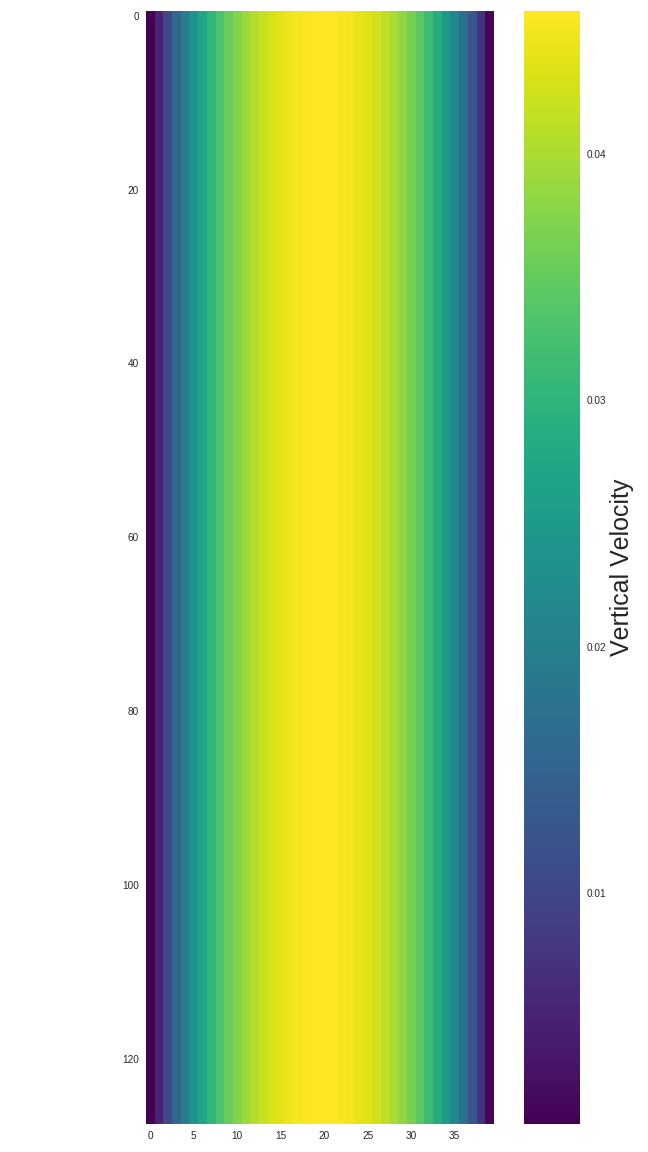
\includegraphics[height=.8\textwidth]{figures/pois_flow.png}
	\caption{Flow through a long cylindrical pipe with a no slip condition enforced at the walls, and a small downward gravitational force. Note how a parabolic distribution of velocity is developed, indicating that the simulation is capturing the theory.}
	\label{fig:pois_flow}
\end{figure}
\begin{figure}
	\centering
	\begin{subfigure}[b]{.49\textwidth}
		\centering
		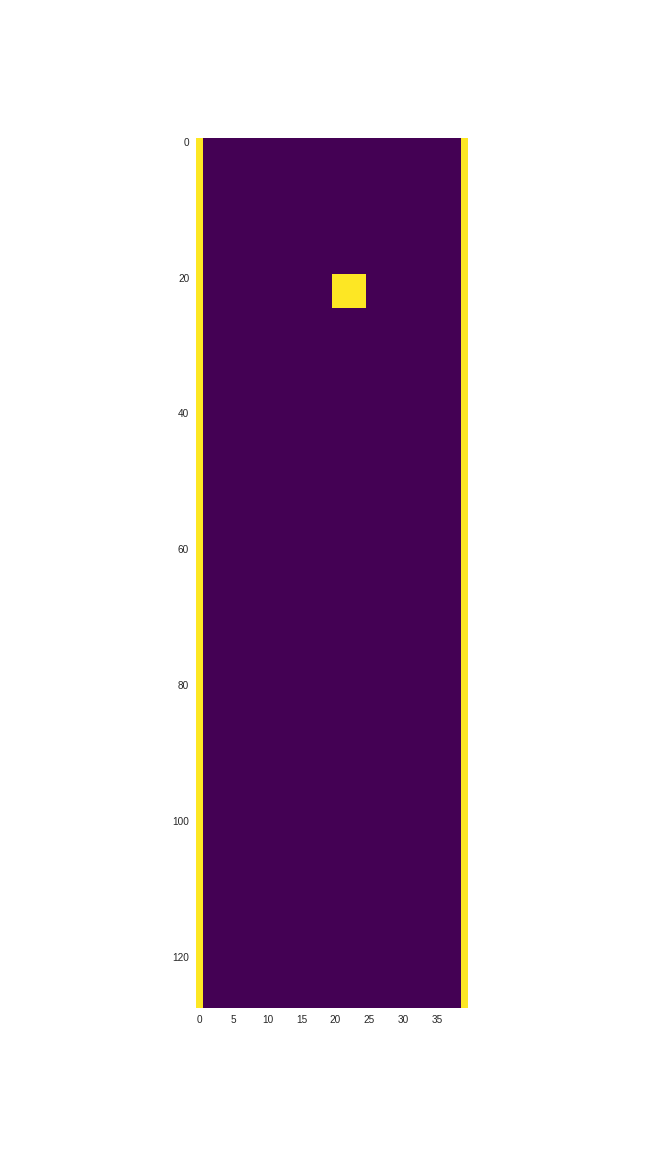
\includegraphics[width=\linewidth]{figures/box_boundary.png}
		\caption{}
		\label{fig:box_boundary} 
	\end{subfigure}
{\tiny {\tiny }}	\begin{subfigure}[b]{0.49\textwidth}
		\centering
		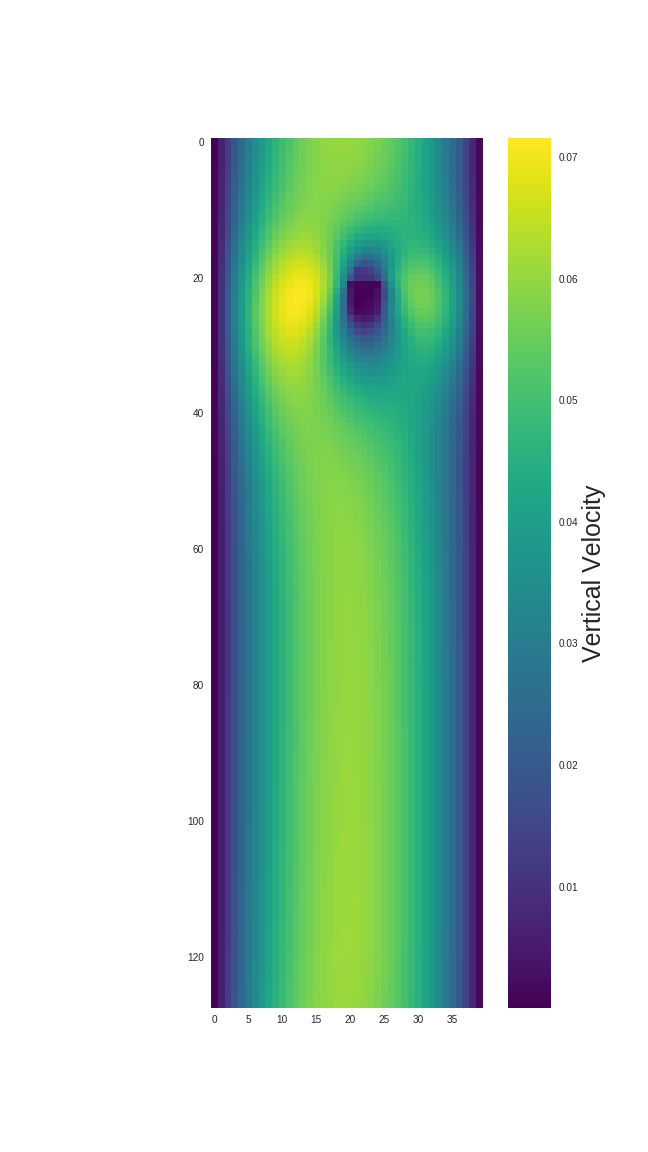
\includegraphics[width=\linewidth]{figures/box_boundary_result.png}
		\caption{}
		\label{fig:box_boundary_result}
	\end{subfigure}
	\caption[]{(a) The boundary used. Yellow cells are boundary cells while purple cells are open to flow. (b) The vertical velocity established after 500 time steps under the influence of a small vertical gravitational force. Even with the box in the middle of the flow path the simulation does not explode. The same code was used here as in Figure \ref{fig:pois_flow}, but a different array of boundary conditions was passed to it, demonstrating the ease of implementing complex boundary conditions with the lattice boltzman method.}
	\label{fig:box_boundary_all}
\end{figure}
\begin{figure}
	\centering
	\begin{subfigure}[b]{.49\textwidth}
		\centering
		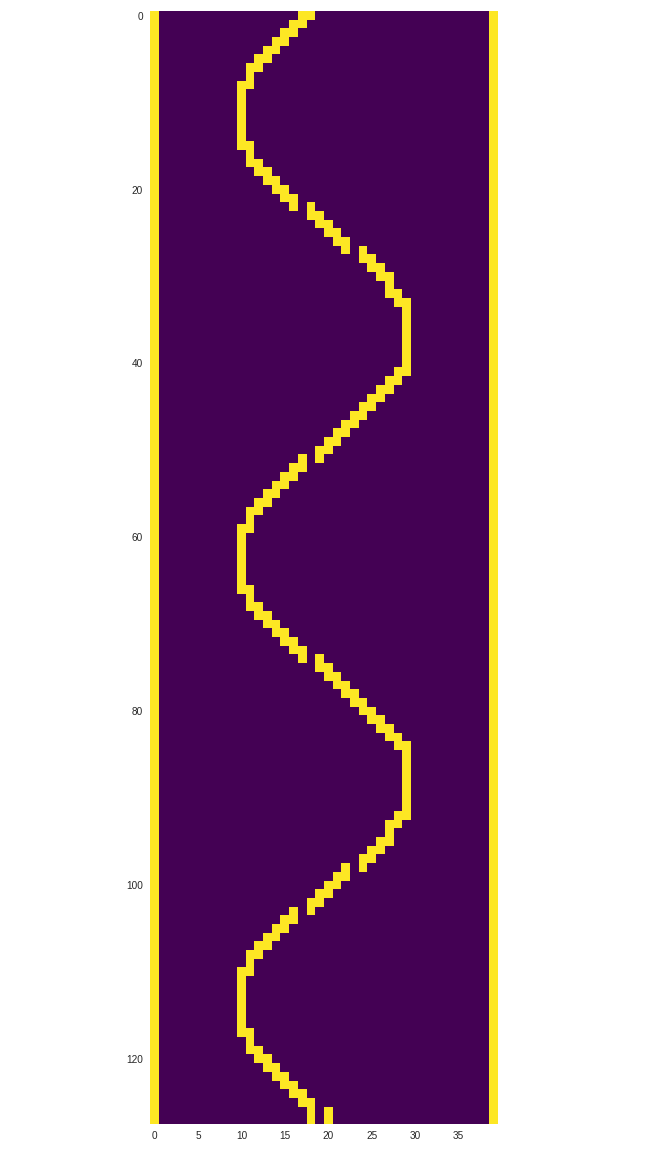
\includegraphics[width=\linewidth]{figures/sin_boundary.png}
		\caption{}
		\label{fig:sin_boundary} 
	\end{subfigure}
	\begin{subfigure}[b]{0.49\textwidth}
		\centering
		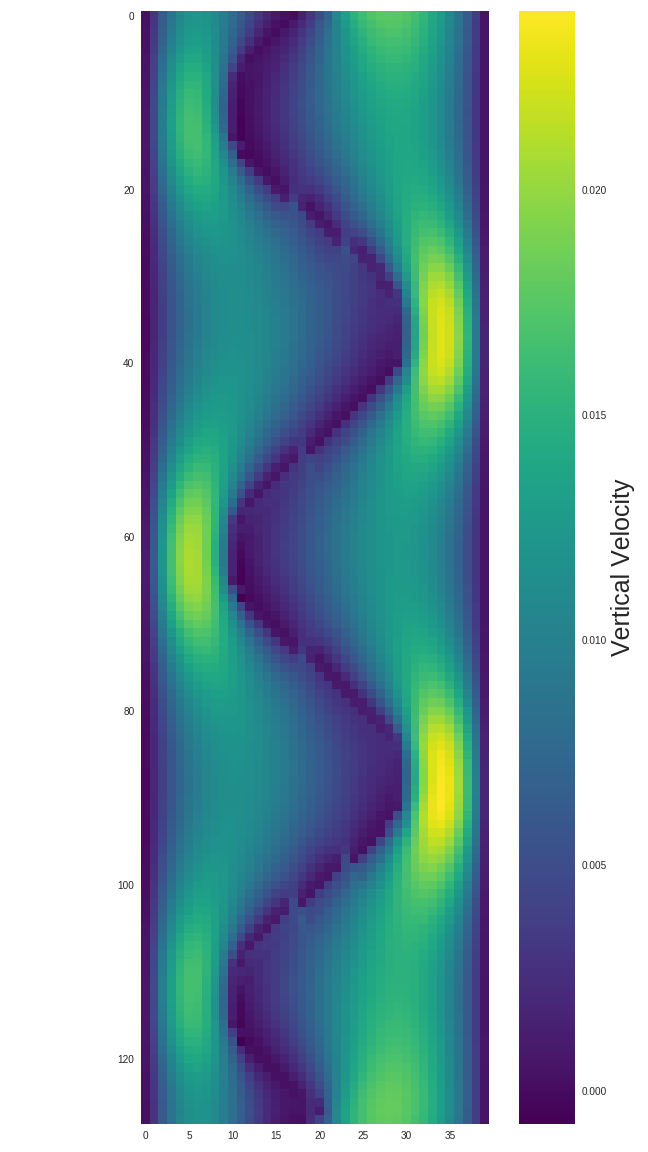
\includegraphics[width=\linewidth]{figures/sin_boundary_result.png}
		\caption{}
		\label{fig:sin_boundary_result}
	\end{subfigure}
	\caption[]{(a) The boundary used. Yellow cells are boundary cells while purple cells are open to flow. (b) The vertical velocity established after 500 time steps under the influence of a small vertical gravitational force.}
	\label{fig:sin_boundary_all}
\end{figure}

\section{Multiphase Flow}
The Lattice Boltzmann method can also be used to simulate multiphase flows. One method of doing this is to follow the method of Shan and Chen \cite{SC}, and modify the velocities used to calculate the equilbirum distributions by a forcing term $F$. Consider $f^{eq}_{\alpha}$ as a function of the velocity at the grid point $\alpha$: $\boldsymbol{u}_{\alpha}$ in the absence of a forcing term. Then we will instead use $\boldsymbol{u}^{eq}_{\alpha}= \boldsymbol{u}_{\alpha}+\frac{\tau F_{\alpha}}{\rho}$, to calculate $f^{eq}_{\alpha}$. We define the force term as:
\begin{equation}
	F_{\alpha} = -G \psi(\boldsymbol{x})\Sigma_i w_i\psi(\boldsymbol{x}+\boldsymbol{e}_i\Delta t)\boldsymbol{e}_i
	\label{eq:forcing}
\end{equation}
where $w_i$ are the lattice weights, $e_i$ the lattice velocities, and $\psi$ is defined differently depending on the model of the physical interactions. The model used here, originally defined by Shan and Chen is:
\begin{equation}
\psi(\rho) = \rho_0(1-\exp(-\rho/\rho_0)).
\end{equation}


The algorithm then is:
\begin{enumerate}
	\item Perform Streaming
	\item Calculate Macroscopic quantities
	\item Modify velocities in accordance with Eq \ref{eq:forcing}
	\item Calculate $f^{eq}$ and relax all lattice points toward it.
\end{enumerate}

I implemented this algorithm using Python and the numerical python library NumPy.

\subsection{Efficiency}
Though Python has a reputation of being incredibly slow these simulations show that this is not entirely warranted. Taking Professor Falcucci's multiphase Fortran code as a baseline for a reasonable runtime we can qualitatively consider the the speed of my Python code. For this comparison I removed the lines of Prof Falcucci's code that output debug info, diagnostics and wrote out each time step to a file. Similarly in the Python code the only output was the final state of the simulation and any calculated values such as the $\Delta P$ for the Laplace test. Under these conditions I found that my moderately optimized Python (with the help of NumPy) had a runtime that was only 2x that of the Fortran. This is certainly slower but, much less of the normally expected 100-1000x \cite{speed} slow down of python relative to Fortran.

\subsection{Random Initial Conditions}
With initial conditions on a square grid with periodic boundary conditions the system evolves to bubbles as expected. The result of such a simulation after 500 time steps can be seen in Figure \ref{fig:muphase_randinit}

\begin{figure}
	\centering
	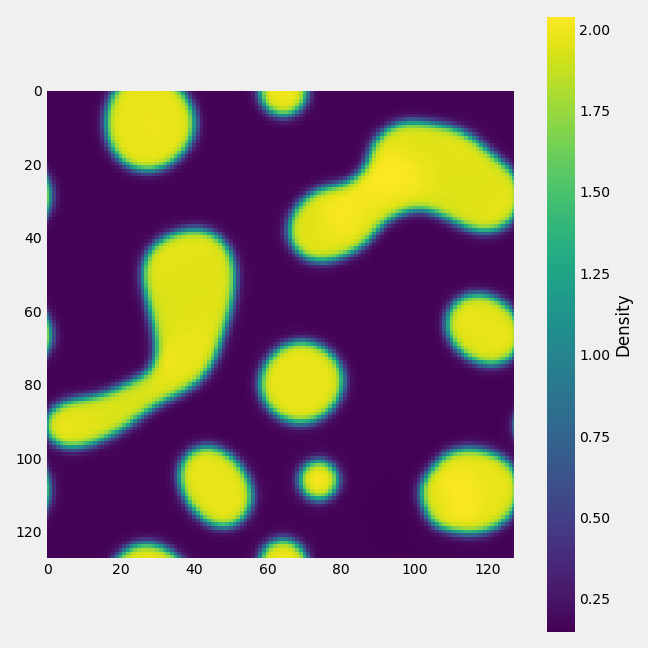
\includegraphics[width=.6\textwidth]{figures/muphase_randinit.png}
	\caption{Density values on a 128x128 grid that was initialized to a spread of random values around $\rho=.69$}
	\label{fig:muphase_randinit}
\end{figure}

 
\subsection{Laplace Test}
If we intialize the simulation with a dense droplet in the center of a less dense gas then we can test our simulation by checking the Laplace equation:
\begin{equation}
\Delta p = \frac{\gamma}{R},
\end{equation}
in which $\Delta p$ is the difference in pressure between the droplet and the gas, and $R$ is the final radius of the droplet. To do this the simulation was initialized as in Figure \ref{fig:laplace_init}, and propagated forward 10000 time steps to achieve equilibrium. The pressure was then calculated as
\begin{equation}
P(\boldsymbol{x}) = \frac{1}{c_s}(\rho(\boldsymbol{x})+.5*G*\psi(\boldsymbol{x})^2),
\end{equation}
where $c_s = \frac{1}{\sqrt{3}}$. The radius can be calculated by solving for R in:

\begin{equation}
\pi R^2 * \rho_{drop} = \text{Mass}_{drop},
\end{equation}
using $ \text{Mass}_{drop} = \text{Mass}_{total}-(\# grid points)*\rho_{min}$, which assumes that the gas surrounding the droplet is all at $\rho_{min}$, we can calculate the radius as:
\begin{equation}
R = \left(\frac{ \text{Mass}_{total}-(\# grid points)*\rho_{min}}{\pi \rho_{drop}}\right)^\frac{1}{2}.
\end{equation}

By varying the value of G, and consequently the surface tension, and radius we can plot $\Delta P$ vs $\frac{1}{R}$ and should expect to see a line of slope $\gamma$. In practice I encountered some difficulty with this. The first issue is that for values of G with $|G|<4.7$ the droplet was unstable and decayed to live on the corners of the simulation as in Figure \ref{fig:muphase_G_46.png}. When considered with the periodic boundary conditions it is clear that there is still a single droplet, however, its positioning across boundaries would have a required a tweaked algorithm to calculate the pressures. Consequently I omitted these simulations. 

Of greater concern is that, as in Figure \ref{fig:laplace_test}, I did not find a linear relationship between $\Delta P$ and $\frac{1}{R}$. This issue was not unique to my implementation, the values for Radius and pressure that I generate are in agreement with the values from Prof. Falcucci's code for the same initial conditions. 

\begin{figure}
\begin{subfigure}[t]{.49\textwidth}
	\centering
	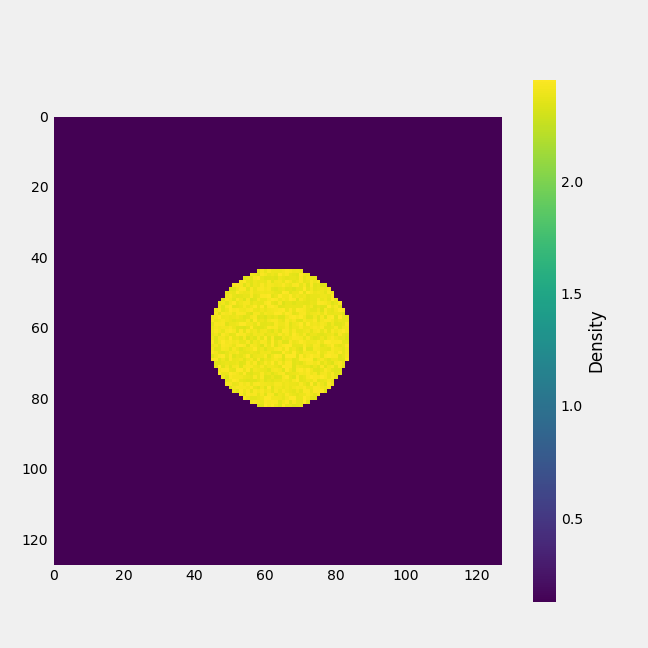
\includegraphics[width=\textwidth]{figures/laplace_init.png}
	\caption{}
	\label{fig:laplace_init}
\end{subfigure}
\begin{subfigure}[t]{.49\textwidth}
	\centering
	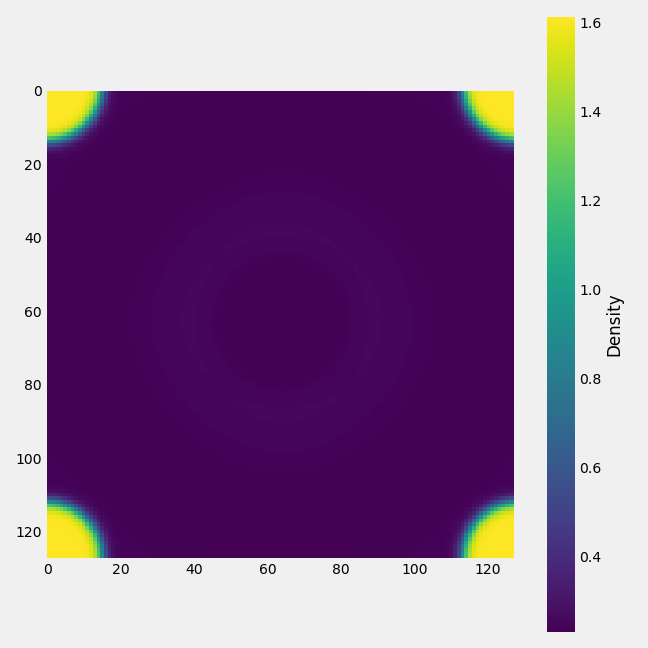
\includegraphics[width=\textwidth]{figures/muphase_G_46.png}
	\caption{}
	\label{fig:muphase_G_46.png}
\end{subfigure}
\caption{(a) Typical initial condition used for the Laplace test. There is a dense droplet in the center within which the value of density has a random 1\% variation.  (b) Density distribution after many time steps from the initial condition in Figure \ref{fig:laplace_init} when using a value of $G=-4.7$. This was not unique to the Python code, professor Falcucci's code also produced this result. This and runs with values of G that produced similar results were excluded from the Laplace test calculations.}
\end{figure}

\begin{figure}
	\centering
	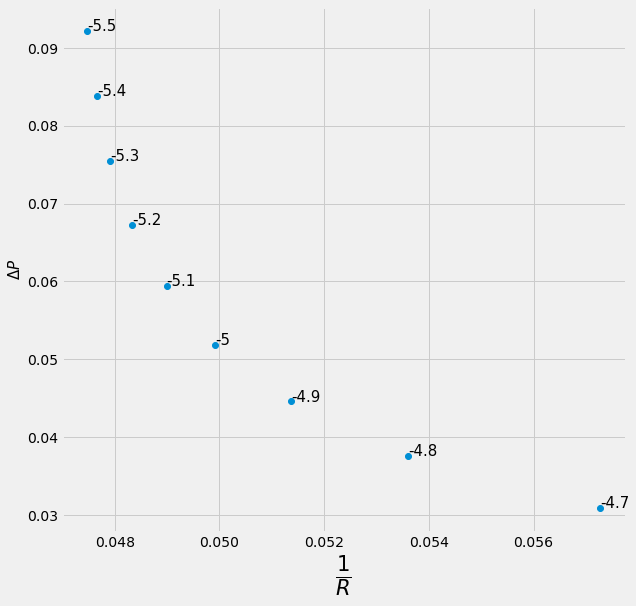
\includegraphics[width=.7\textwidth]{figures/laplace_radInit21.png}
	\caption{The relationship I found via the Laplace test is decidedly nonlinear, I am not sure why this is. The points are individually labeled with the value of G used for the corresponding simulation.}
	\label{fig:laplace_test}
\end{figure}
\begin{thebibliography}{99}
	\bibitem{SC} X. Shan and H. Chen, Phys. Rev. E 47, 1815 (1993).
	\bibitem{speed} https://scicomp.stackexchange.com/a/11524

\end{thebibliography}
\end{document}